\chapter{System Model and Requirements}
\label{ch:System Model and Requirements}
Now that an overview of the topic has been provided, the next part will deal with a basic system model and the requirements that will be imposed on the design. The system model gives an overview of the different parties that exist in our shared parking model and their relationships with each other. The subsequent requirement analysis is divided into functional and security requirements. Special attention is paid to ensuring that the design is secure. For us security requirements do not only refer to standard security aspects such as encryption, user authentication and authentification, but in particular to the goal of designing our shared parking system in a way that it has the ability to handle fraud independently. For instance, the system should prevent and punish individual users from scamming other users or the system. Various forms and examples of such fraud will be considered and evaluated. The system design presented in Chapter \ref{ch:Design} will adhere to these requirements. We will now start of with a high-level overview of the shared parking system.

\section{High-level Overview}\label{High-level Overview}
This section gives a high-level overview of the proposed shared parking system and deals with the basic capabilities of the system. The shared parking system adheres to the definition supplied at the beginning. It offers a platform for an online marketplace where both private and business users can rent and lease parking spaces. End users have the opportunity to install an app and participate in the marketplace using their smartphone. This also clarifies the basic capabilities of the system. Every user can offer his own parking spaces for specified periods of time on the platform for rent. Users can also view other users' listings, choose from them and rent those parking spaces. In this system, particular importance is given to handling fraud. The subsequent requirements define the exact framework under which the design was developed. Unlike state-of-the-art shared parking systems, our system will largely do without expensive hardware, which leads to high deployment costs for service providers and users in other systems. In addition, the system should operate mostly without manual intervention by the service provider, thus keeping maintenance costs low. Another unique feature of our system is that it can handle different attacks and fraud. No other shared parking system published, has, to our best knowledge, the ability to deal with all the different cases of fraud we define later on. In contrast to many other access control systems, our system does not aim at preventing unauthorized access of adversaries to parking spaces, but instead incorporates mechanisms to punish misbehaving users. Enforcing access control to parking lots would likely require installation of special equipment on parking lots, which we ruled out above because it would increase deployment costs of the system and raise entrance limits for landlords, which is undesirable. These mechanisms include, for example, a rating module that allows users to rate each other after each rental operation. Also part of those mechanisms is a reporting module that allows users to report adversaries. In addition, there is a module that verifies the validity of reported fraud cases through the service of other users. Finally, there is a module that monitors all processes within the system and calculates a reputation score for every user based on those. This score reflects the trustworthiness of a user.

\section{System Model}\label{System Model}
The following system model, which is depicted in figure \ref{img:system model}, shows the various parties in our \textbf{shared parking system} $SPS$. On the one hand, there is exactly one \textbf{operator} or \textbf{service provider} $SP$. The $SP$ is responsible for the implementation of the design, operating the $SPS$ and making the systems services available to the users. The \textbf{users} $U$ are those who utilize the $SPS$. They can be divided into two roles, whereby a user can be part of both roles at different points in time. On the one hand, there are \textbf{landlords} who own a private \textbf{parking space} $p \in P$ and want to rent it out over a certain period of time. On the other hand, there are \textbf{tenants} who are looking for a free parking space to rent for a specific time period.

This work covers fraud in $SPS$ in detail. In the \textbf{case of fraud}, users take on new roles. On the one hand there is the \textbf{adversary}, who is committing fraud, on the other hand there usually is an \textbf{injured party}, which has a disadvantage caused by the fraud case.

As mentioned in \ref{High-level Overview} we will utilize different modules that deal with those fraud cases. In each of those modules users once again assume different roles.

The rating module deals with \textbf{ratings}. For each rating there is one user who issues, called the\textbf{ rating user} and one user who receives, called the \textbf{rated user}.

The reporting module deals with \textbf{reports}. One report belongs to one case of fraud. For each report there is one user who issues, called the \textbf{reporting user} and one user who receives, called the \textbf{reported user}.

The verification module verifies reports and the corresponding fraud case. Users who verify the reports are called \textbf{inspectors}.

In the reputation module, \textbf{contributions} from all \textbf{participants} of one fraud case are processed. The participants include the reporting user, reported user and the inspectors. A participants' contribution is the information he provides about the fraud case.

All roles are described in more depth in the detailed description of the modules.\\

\begin{figure}
	\centering
	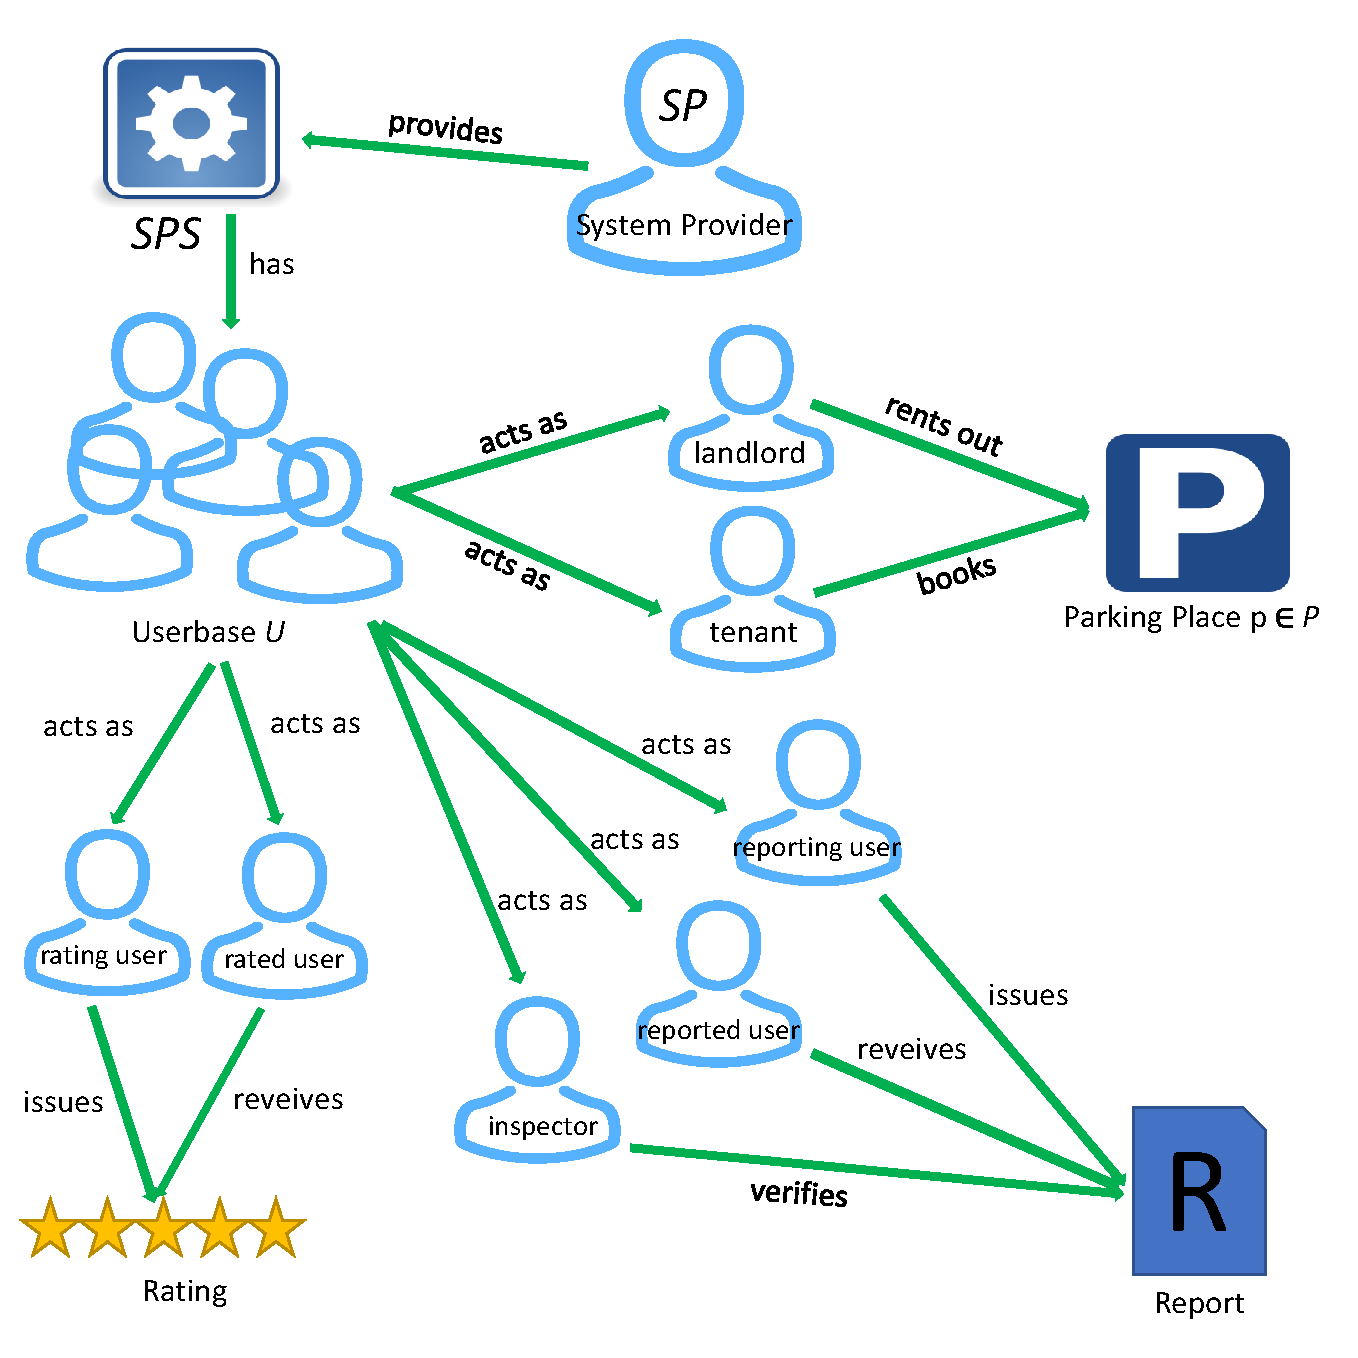
\includegraphics[width=13cm,height=11cm]{logos/system-model-grafik.pdf}
	\caption{System Model}
	\label{img:system model}
\end{figure}

\section{Functional Requirements}
The following will cover the main functional requirements. To keep deployment and maintenance costs low, we require the system to operate with of the shelf hardware autonomously in most situations. We further require different features for our prototype. It must provide users with the basic functions that allow them to rent and let parking spaces. Further features are listed below. 

But there are also areas that do not place any functional requirements. These are aspects to which no special significance is attached to in this work. This includes, for example, all legal matters. On the one hand, this study is in the field of computer science and the author does not have the fundamental knowledge to evaluate and judge legal matters. On the other hand, the legal aspect of a shared parking system involves many and various legal factors, which would exceed the scope of this work. We, for example, would need to think about whats necessary to set up a contract between two online parties or how exactly to punish an adversary by a fine. Nevertheless, attention was paid during the design process to carry out as little legal interference as possible in order to avoid legal difficulties during the realization. A reporting user for example does not need provide any pictures of the adversaries' car on private ground issuing a report to the $SPS$. The functional requirements are depicted below in greater detail.

\subparagraph{Low deployment cost and of the shelf hardware} Neither the operator nor the user should need any additional and expensive hardware. For getting the system to work the user just needs a off-the-shelf smartphone and the operator only needs to provide enough computational power to get the server running. There will be no sensors installed at the parking spots, no additional hardware used for confirming parking time or the likes of that.
\subparagraph{Automatic Processing} Where possible, the $SPS$ should be prevented from requiring manual intervention by the $SP$. The system should be able to run all basic use cases should and may only request manual intervention in exceptional cases. On the one hand this should lead to a fast processing of all inquiries and on the other hand reduce the costs for the $SP$ stemming from employing people for manual tasks.

\subparagraph{Basic functions} The user must be able to book or rent out a parking spaces through the app. This requirement also includes all sub functions necessary (like log-in, registering a car and many more) to achieve this goal.

\subparagraph{Search function via a map} The user must be able to search for parking spaces on a map, where he can input the time and location and available parking spaces get highlighted. 

\section{Adversary Model and Assumptions}\label{sec:Adversary Model and Assumptions}

\subsection{Adversary Model and Classes of Fraud}
When we talk about fraud, we mean a user's ability to scam other users or the system using its normal functionality in order to gain a profit. In many cases, this has a negative impact on other users. There are numerous possibilities for fraud in the system, some of which are mentioned as follows. We will categorize all fraud cases into three different classes. As mentioned in \ref{System Model} we refer to a user who commits fraud as a adversary. Users who are affected by fraud in a negative way will be called injured or injured party. \\

\subparagraph{Class 1} The first class of fraud cases are the result of the general nature of a shared parking system. This class consists of fraud cases where a tenant has booked a parking space, but it is not available when he arrives. There could be different possibilities as to why the parking space is not available, examples of which are the following.
\begin{itemize}
\item adversary parks in a car park, which another user has booked for this time.
\item Tenant overstays his booked parking time.
\item Landlord rents out a parking space, but remains on it himself.
\item Landlord offers the same parking space multiple times.
\item Landlord offers a parking space that does not exist.
\end{itemize}
To deal with these class 1 cases, we will introduce various modules, such as a report module and a reputation module, which enables detection of the attacks described above. As we will see later, Class 1 cases can be handled by our system without manual intervention. 

\subparagraph{Class 2} The reputation module helps to deal with class 1 cases of fraud, however it itself is subject to a new series of fraud cases. We group these new fraud cases into class 2. All well known attacks in this area are described in \cite{mousa2015trust} and are applied to our system as follows:
\begin{itemize}
\item \textbf{Corruption attack:} An adversary unintentionally or deliberately sends corrupted data and information. An example of a corruption attack is when a reporting user enters an incorrect license plate number for the reported user.
\item \textbf{On-off attack:} An attacker alternates between malicious and genuine behavior. This is particularly difficult to detect when the transition appears to occur randomly.
\item \textbf{Re-entry attack:} An adversary tries to white wash his trust value by rejoining the system with a new identity. In our system this corresponds to a new registration of an existing user.
\item \textbf{Collusion:} Several adversaries act together and execute attacks collectively. Joint attacks have a greater impact on the system and are harder to detect than acting independently.
\item \textbf{Sybil attack:} This is an extension of the re-entry attack. An adversary creates multiple identities or accounts within the system and utilizes them in a collusion attack.
\item \textbf{Reputation lag exploitation:} The adversary uses the period between his first attack and the evaluation and corresponding downgrading of his trust value to launch a large number of attacks.
\item \textbf{GPS spoofing attacks:} The adversary tampers with the GPS location of his device.
\item \textbf{Unfair ratings:} The adversary does not rate another user according to his genuine opinion.
\item \textbf{Bad mouthing or negative discrimination attack:} The adversary raises false accusations or assigns a bad rating to a genuine user.
\item \textbf{Ballot stuffing or positive discrimination attack:} The adversary does not report misbehaviour or assigns a good rating to a malicious user.
%User tries to impose costs on to the system by doing false reports. adversary pretends to be the injured party. adversary accuses another user of fraud.
\end{itemize}
We shall see that Class 2 cases can also be dealt with mostly without manual intervention by using a robust reputation module. 

\subparagraph{Class 3} While the first two classes cover the main and most frequent cases of fraud, there are others. Class 3 cases differ from the other classes in that it will not be possible to solve them without manual intervention. These are exceptional cases that occur only in low frequency. Examples are given below.
\begin{itemize}
\item Landlord rents out parking spaces that they do not own themselves.
\item Tenant cancels booking of a parking space without paying.
\end{itemize}
For this class of fraud cases, we will also show methods of dealing with them.\\

Most of these attacks can only be performed by registered users. In contrast, however, there is a case of fraud, which can also be carried out by persons outside the system. A parking offender who occupies a booked, private parking space does not necessarily have to be registered in the system. Dealing with this problem is not the main focus of this work, but a suggestion on how to deal with it when realizing the system will be provided in section \ref{sec:Comments on the realization}.

\subsection{Assumptions}\label{sec:Assumptions}
In the following we specify assumptions that apply to our system.\\

\subparagraph{Attacker collaboration} We assume that adversaries can not only attack the system on their own, but collaborate with other adversaries to jointly start and carry out attacks. We will show that even under this assumption the $SPS$ can protect itself from  the attacks described above.

\subparagraph{Sufficient parking spaces} We assume that there are always enough parking spaces available for compensation. The assumption is reasonable, since if the system has low occupancy levels, a suitable free parking space can always be found. If this is not the case, there will always be landlords  who offer their parking spaces for a particularly expensive and overpriced costs. These places will still be vacant even in situations where almost all capacities are occupied. These are parking spaces that are still available for use as compensation for injured parties, even when there is a high level of occupancy. 

\subparagraph{Majority assumption} We assume that the majority of users in our system are acting according to the rules, meaning that there are always a maximum of 50 percent adversaries. Even under the \textit{attacker collaboration} assumption it is reasonable to believe that there will be plenty of genuine users that use the system for parking and not for fraud as this is a typical assumption for distributed systems (e.g. \cite{benenson2004secure}, \cite{nojoumian2014efficient}, \cite{avoine2005gracefully}). One can expect that the majority of people are genuine, especially when they know that offenses are being punished hard. We further offer an opportunity to report inadvertent misdemeanors, in order to prevent major penalties, by yourself, which should prevent inadvertent misdemeanors by genuine users.\\

\section{Security Requirements}\label{Security Requirements}
The following will cover the main security requirements in detail. On the one hand, requirements are made on information security and on the other hand, requirements are mode on how to deal with fraud in the shared parking system. From the information security standpoint, we specify that several requirements must apply in a realization of the $SPS$. Data traffic over the internet should always be encrypted, passwords should never be stored in plain text, user mail must be confirmed after registration and much more. These information security requirements are long standing standard and thus not need to be further discussed in the design chapter. They can be implemented independently from the design. They are also not put into practice in our prototype, but need to be implemented if one wants to bring the system to the market.

Then there are also areas that do not place any special requirements on security. Even without a shared parking system, attacks on the private parking infrastructure are possible. One person can for example park their car in another person's private car park. The injured party then has two options, both of which can have strong disadvantages for him. He could call the towing service, hope that the adversary has not left by its arriving time or he will have to bear the expensive towing fees himself. The other option is to do nothing and look for a new parking space for himself. Problems as these, which are already present, do not need to be solved. However, it can be seen as a bonus to prevent such problems with good design choices for the $SPS$.\\

The system must be able to handle all these cases of fraud mentioned in the adversary model above successfully. In the following we will define what we mean by 'successful handling'. We therefore set requirements that must be met for the various cases of fraud.
\subparagraph{Fraud Prevention} The design of the system should be such that fraud is fundamentally prevented. If this is not possible in all cases, it should be ensured that it is not worth the effort for the adversary or that adversaries are quickly discovered. This is where the second point comes into play.
\subparagraph{Fraud Detection} The system should be able to detect fraud. This includes, on the one hand, the simple recognition of fraud and, on the other hand, the ability to correctly identify the adversary. The later is particularly important for the next point.
\subparagraph{Fraud Punishment} The design should be such that a adversary can be punished by the system. After a adversary is detected, the system should always be able to penalize him. Punishment can also support the first requirement by acting as a deterrent for fraud.
\subparagraph{Fraud Compensation} Finally, the system should be able to compensate an injured party. If injured are compensated, there is no need for genuine users to worry about fraud and thus enhances the attractiveness of the system.\\